% !TeX root = ../Aquila_Pflichtenheft.tex

% Chapter7
\chapter{Benutzerschnittstelle} \label{chapter:benutzerschnittstelle}

Die Benutzeroberfl�che von Aquila besteht aus Website zur Steuerung und Information des Benutzers, die im Folgenden spezifiziert wird.\footnote{Die Bezeichnungen, sowie das aktuelle Design der beschriebenen Bereiche sind vorl�ufiger Natur und k�nnte sich im Verlauf des Projektes noch �ndern.}\\
	Die Website informiert �ber aktuelle Kennzahlen und Daten zu verwalteten Aktien, zeigt Performanceinformationen des verwalteten Portfolios an und stellt Charts dar, mit deren Hilfe historische Entwicklungen interpretiert werden k�nnen und der Algorithmus aus menschlicher Sicht verst�ndlicher und �bersichtlicher wird. Au�erdem besitzt die Website eine zentrale Steuerfunktion, d.h. Einstellungen, Ver�nderungen und Parameter k�nnen �ber diese an die Software weitergegeben werden.\\
	Bestandteile der Website sind eine Seite zur �bersicht �ber verwaltete Aktien, wo diese sowohl bearbeitet, als auch neue hinzugef�gt werden k�nnen. Eine Seite gibt Informationen �ber die Performance des Portfolios b.z.w. auch �ber den Algorithmus. Im Einstellungsbereich sind Einstellungen zu Trading-relevanten Themen, wie beispielsweise Voreinstellungen f�r die Cut-Loss-Schwelle, sowie Accounteinstellungen vorzunehmen. Abbildung \ref{fig:web_aktien} stellt ein Grundger�st der Aktien-Seite dar. �ber die Suchfunktion k�nnen neue Aktien gefunden und hinzugef�gt werden. Die Tabelle zeigt die wichtigsten Daten zu den verwalteten Aktien an. Durch Klick auf eines der Symbole gelangt der Benutzer zur Informationsseite dieser Aktie, wo Charts und  jeweilige Performance-Informationen pr�sentiert werden.\\

\begin{figure}[htb]
	\centering
		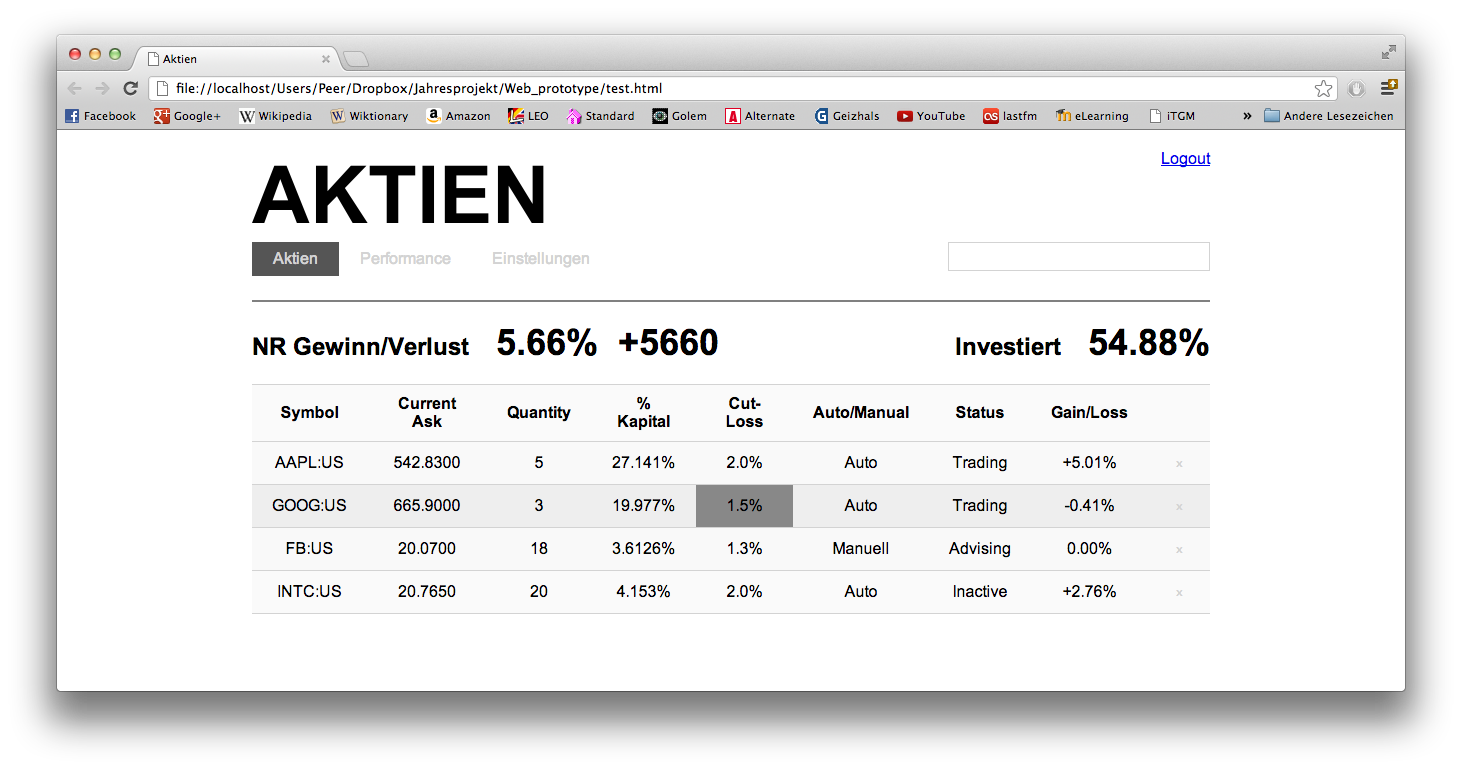
\includegraphics[width=1\textwidth]{graphics/benutzerschnittstelle/web_aktien.png}
	\caption{Website-Grundger�st}
	\label{fig:web_aktien}
\end{figure}

\begin{minipage}{\textwidth}
	Die Seitenstruktur weist folgende Struktur auf:
	\begin{itemize}
		\item{Aktien}
			\begin{itemize}
				\item{Symbolinformation}
			\end{itemize}
		\item{Performance}
		\item{Einstellungen}
		\begin{itemize}
			\item{Trading}
			\item{Account}
		\end{itemize}
	\end{itemize}
\end{minipage}\\
\\
\\
/B10/ \textbf{Grafisches Design}\\
Das Design soll modern und schlicht sein, wodurch eine flotte Bedienung erreicht wird und Informationen schnell aufgenommen werden k�nnen. Durch einfache Farbkontraste werden auf simple Art und Weise Hinweise, wie der Status der Aktie oder m�gliche Benutzerinteraktionen, angezeigt.\\
\\
/B20/ \textbf{Wechsel der Betrachteten Aktie}\\
Im Informationsbereich kann der Benutzer aus den Aktien, die er aktuell handelt, eine ausw�hlen, f�r die anschlie�end alle Informationen und Charts angezeigt werden.\\
\\
/B30/ \textbf{Anzeige der Performance}\\
Die Performance des Algorithmus wird in Zahlen f�r die betrachtete Aktie f�r eine bestimmte Zeitperiode angezeigt.\\
\\
/B40/ \textbf{Charts}\\
Zur Information des Benutzers soll als Chart die Preisentwicklung der betrachteten Aktie, sowie die \glspl{ma} und sowohl Einstiegs-, als auch Ausstiegspunkte des Algorithmus angezeigt werden. Dies soll sowohl kurz-, als auch langfristig m�glich sein.
Au�erdem soll das aktuelle Ergebnis des Algorithmus angezeigt werden.